\documentclass[10pt, conference, compsocconf]{../IEEEtran}
\usepackage{xltxtra}
\usepackage{subfig}
\usepackage{booktabs}
\usepackage{amsmath}
\usepackage{flushend}
\usepackage[numbers,sort&compress]{natbib}
\setmainfont{Times New Roman}

\begin{document}

\title{idock: A Multithreaded Virtual Screening Tool for Flexible Ligand Docking} % can use linebreaks \\ within to get better formatting as desired
\author
{
\IEEEauthorblockN
{
Hongjian Li, Kwong-Sak Leung and Man-Hon Wong
\IEEEauthorblockA
{
Department of Computer Science and Engineering, Chinese University of Hong Kong, Hong Kong, P.R. China\\
\{hjli, ksleung, mhwong\}@cse.cuhk.edu.hk
}
}
}
\maketitle

\begin{abstract}

AutoDock Vina is a competitive protein-ligand docking tool well known for its fast execution and high accuracy. Nevertheless, when docking a massive number of ligands, Vina has to be run multiple times, repeating receptor parsing and grid maps building over and over again. There are tremendous requests for revising Vina to reuse precalculated data and incorporate built-in support for virtual screening. Hence we developed idock, inheriting from AutoDock Vina the accurate scoring function and the efficient optimization algorithm, and significantly improving the fundamental implementation and numerical model for even faster execution. idock achieves a speedup of 3.3 in terms of CPU time and a speedup of 7.5 in terms of elapsed time on average. idock is free and open source, available at https://GitHub.com/HongjianLi/idock.

\end{abstract}

\begin{IEEEkeywords}

bioinformatics, chemoinformatics, drug discovery, protein-ligand docking, virtual screening, multithreading

\end{IEEEkeywords}

\section{Introduction}

As the X-ray crystallography technology evolves, more and more structures of biological macromolecules at atomic level have been revealed and deposited into the world's largest repository Protein Data Bank (PDB) \cite{539,537}. This rapid evolution catalyzes the development of various protein-ligand docking tools for structure-based drug discovery.

Protein-ligand docking is a method which predicts the preferred conformation of a small ligand when bound to a macro protein to form a stable complex. It also predicts the binding affinity in terms of free energy. The lower the free energy, the higher the binding affinity. Very often, the target protein is a viral enzyme of interest, and the small organic ligands that are predicted to inhibit the viral enzyme are what we want to discover. Structure-based virtual screening is simply a massive version of docking. It docks a database of drug-like ligands to a target, ranks them according to their predicted binding affinity, and shortlists the best ones for further investigation.

Among the many protein-ligand docking programs, AutoDock Vina \cite{595} (hereafter Vina for short) is a competitive one. It is free and open source. It runs faster than its predecessor AutoDock4 \cite{596} by an order of magnitude \cite{556}. First released in 2010, Vina has been cited by over 260 publications according to Google Scholar and adopted by quite many researchers \cite{609}, demonstrating its popularity.

\section{Motivation}

Vina is a popular and competitive protein-ligand docking tool well known for its fast execution and high accuracy. Nevertheless, Vina is optimized for single-ligand docking rather than virtual screening. When it comes to docking a large pool of ligands, Vina has to be invoked multiple times, repeatly parsing the same receptor and creating the same grid maps, and thus degrading performance. There are enormous requests from community for modifying and recompiling Vina to make it support virtual screening in a superfast manner by reusing receptor and grid maps. We were motivated by the desire to provide built-in support for virtual screening and therefore developed idock. Moreover, we incorporated many implementation tricks to further speedup idock and utilized idock to address a real life drug discovery problem.

\section{Problem Definition}

At present, 25 drugs have been approved by US Food and Drug Administration (FDA) for the treatment of HIV/AIDS \cite{300}. Among them, tenofovir disoproxil fumarate (TDF) is for the treatments of both human immunodeficiency virus (HIV) and hepatitis B virus (HBV). It is a nucleoside inhibitor of reverse transcriptase (RTs) of HIV and HBV. A considerably greater proportion of HBV+ recipients of TDF 300 mg once daily achieves a complete response at week 48 than oral adefovir dipivoxil 10 mg once daily \cite{165}. TDF is also generally less expensive and more convenient to administer, as it does not require dosing on an empty stomach \cite{159}.

However, clinical feedback reveals that TDF exhibits strong side effects, causing osteomalacia and mitochondrial toxicity on the renal proximal tubule \cite{185}. Justification of the side effects shows that 1) S-Adenosyl-L-homocysteine hydrolase (SAHH), a highly conserved ubiquitous enzyme that catalyzes the hydrolysis of S-Adenosyl-L-homocysteine (SAH) into adenosine and homocysteine, is affected, leading to defect in DNA methylation-dependent gene silencing \cite{182}. SAHH inhibitor has signs of immunosuppressive activity \cite{183}. 2) Adenosine deaminase (ADA) is inhibited, resulting in reduced breakdown of adenosine from food and decreased turnover of nucleic acids in tissues \cite{999}. ADA inhibitor 2′-deoxycoformycin (dCF) shows signs of hepatic and adrenal toxicity \cite{187}. 3) Purine nucleoside phosphorylase is also inhibited. Figure \ref{fig:EnzymaticAssay}, reprinted from Sigma-Aldrich Co., shows the enzymatic assay of the above three enzymes, which break down SAH eventually into uric acid inside human body. Table \ref{tab:TanimotoCoefficients} indicates that TDF is structurally similar to the inhibitors of SAHH, ADA, and PNP, hence TDF is likely to inhibit them in addition to HIV RT. For HIV-infected or HBV-infected patients who take TDF as the primary drug, it is unfortunate that these three essential enzymes are simultaneously inhibited by TDF.

\begin{figure}
\centering
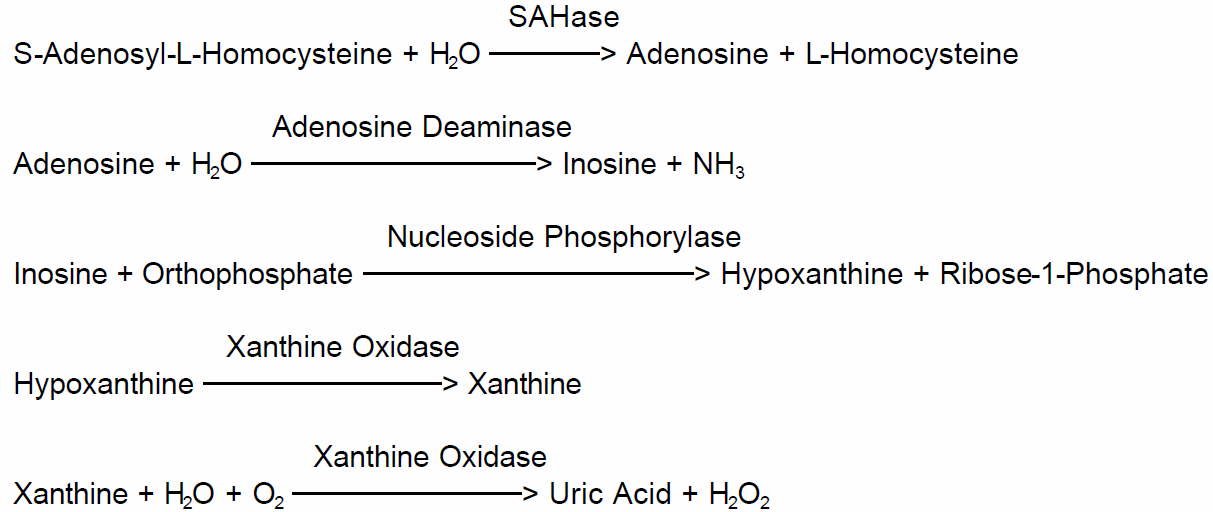
\includegraphics[width=\linewidth]{Figures/EnzymaticAssay.png}
\caption{Enzymatic assay of SAHH. Figure reprinted from Sigma-Aldrich Co.}
\label{fig:EnzymaticAssay}
\end{figure}

\begin{table}
\centering
\begin{tabular}
{rcc}
\toprule
& Scitegic ECFP4 fingerprint & Daylight fingerprint\\
\midrule
HIV RT inhibitor & 1.00 & 1.00 \\
  SAHH inhibitor & 0.51 & 0.70 \\
   ADA inhibitor & 0.42 & 0.75 \\
   PNP inhibitor & 0.51 & 0.76 \\
\bottomrule
\end{tabular}
\caption{Tanimoto coefficients between TDF and the inhibitors of HIV RT, SAHH, ADA, and PNP using the Scitegic ECFP4 and Daylight fingerprints through the SEA database \cite{380}.}
\label{tab:TanimotoCoefficients}
\end{table}

The problem is to discover a few promising compounds that inhibit HIV RT only, minimizing toxicity without affecting SAHH, ADA, or PNP. From the computational perspective, it is equivalent to shortlisting candidates from existing ligand databases such that they bind to HIV RT with a higher affinity and bind to SAHH, ADA, and PNP with a lower affinity. This can be done by protein-ligand docking.

\section{Method}

Vina is a popular protein-ligand docking tool. Based on Vina, we developed a fast virtual screening tool called idock, and used it for the discovery of compounds that inhibit HIV RT without affecting SAHH, ADA, or PNP. idock borrows many great ideas from Vina, and meanwhile introduces its own innovations. Its input includes a rigid receptor, a flexible ligand, and a box used to restrict the conformational space to a particular binding site. Its output includes predicted conformations and their predicted free energies in kcal/mol. idock consists of two basic components, a scoring function to predict the binding affinity, and an optimization algorithm to explore the conformational space.

Figure \ref{fig:idockFlowchart} shows the overall flowchart of idock. During initialization, idock precalculates the scoring function for all possible combinations of atom type pairs and interatomic distances. It parses the receptor and determines the atom types with the aid of residue sequence, and creates a thread pool to hold reusable threads. Then it enters a loop and fetches a ligand from a user-specified input folder to perform docking. It parses the ligand and determines the atom types with the aid of branch information, and meanwhile automatically detects and deactivates inactive torsions. It builds grid maps of granularity 0.15625 \AA\ by default on the fly by multithreading, and distributes multiple independent Monte Carlo tasks to the thread pool for concurrent execution. Then it merges the conformations from separate threads and clusters them with RMSD 2.0 \AA, and dumps them to the user-specified output folder and displays the predicted free energy on screen. It proceeds with the next ligand automatically until all are docked. Finally it destroys the thread pool and releases memory resources.

\begin{figure}
\centering
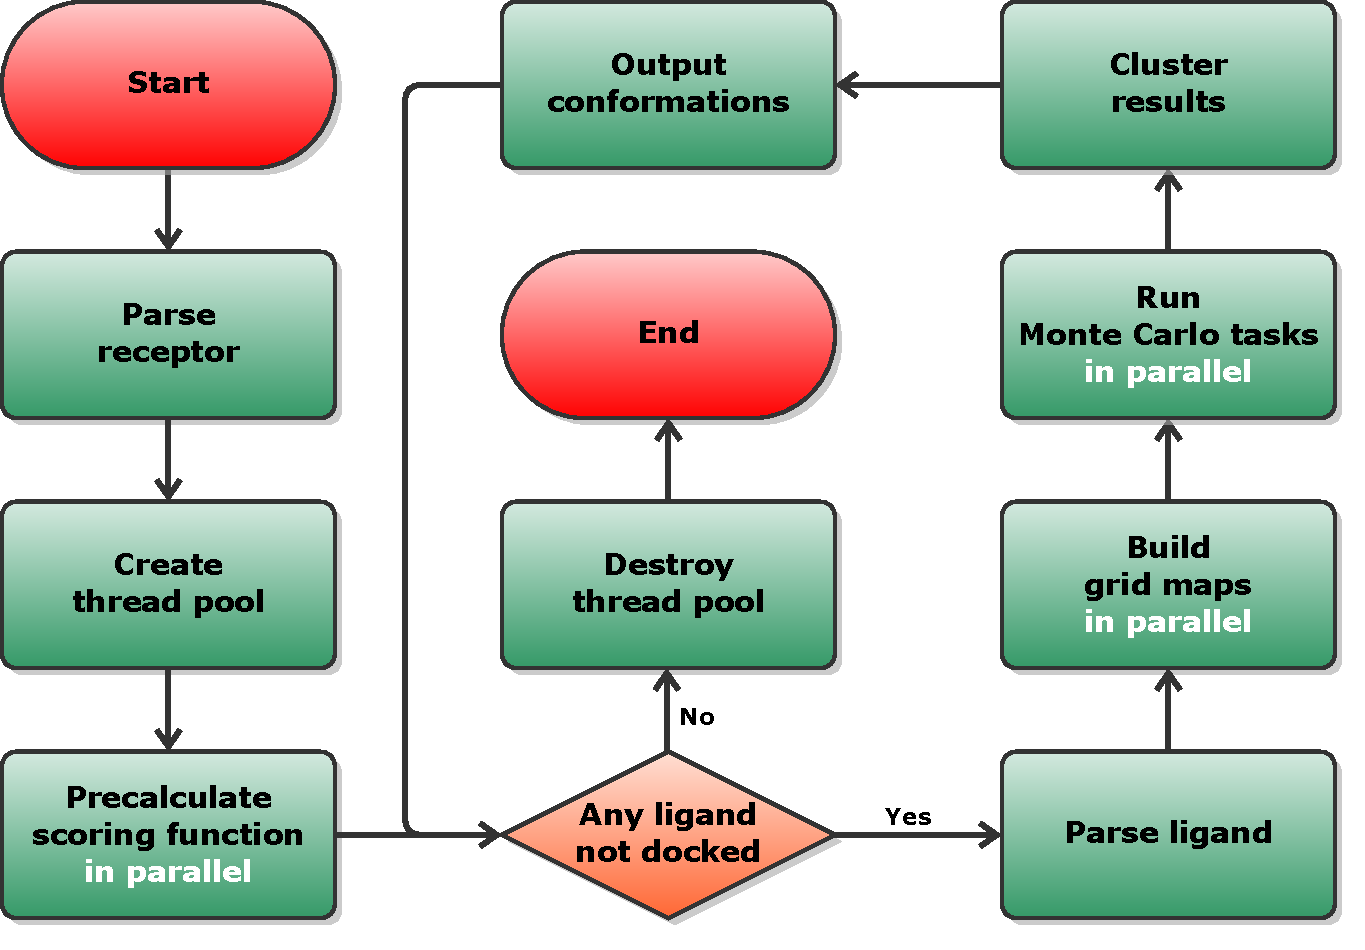
\includegraphics[width=\linewidth]{Figures/Flowchart.pdf}
\caption{Flowchart of idock.}
\label{fig:idockFlowchart}
\end{figure}

\subsection{Scoring Function}

Both idock and Vina share exactly the same scoring function, which is made up of a conformation-dependent part and a conformation-independent part. The conformation-dependent part is a weighted sum of five terms over all the pairs of atom $i$ and atom $j$ that can move relative to each other. It is calculated from equations \eqref{eqn:e} and \eqref{eqn:eij} where $t_i$ and $t_j$ are the atom types of $i$ and $j$ respectively, and $r_{ij}$ is their interatomic distance. The five terms are calculated from equations \eqref{eqn:Gauss1} to \eqref{eqn:HBonding} where $d_{ij}$ is the surface distance calculated from equation \eqref{eqn:dij} where $R_{t_i}$ and $R_{t_j}$ are the Van der Waals radii of $t_i$ and $t_j$ respectively. All the units are in \AA. The weighting coefficients and the cut off at $r_{ij}$ = 8 \AA\ of the five terms are borrowed from Vina. The optimization algorithm attempts to find the global minimum of $e$ and other low-scoring conformations, which it then ranks.
\begin{equation}
\label{eqn:e}
e = \sum_{i < j} e_{ij}
\end{equation}
\begin{eqnarray}
\label{eqn:eij}
e_{ij} &=& (-0.035579) * Gauss_1(t_i, t_j, r_{ij}) \nonumber \\
       &+& (-0.005156) * Gauss_2(t_i, t_j, r_{ij}) \nonumber \\
       &+& (+0.840245) * Repulsion(t_i, t_j, r_{ij}) \nonumber \\
       &+& (-0.035069) * Hydrophobic(t_i, t_j, r_{ij}) \nonumber \\
       &+& (-0.587439) * HBonding(t_i, t_j, r_{ij})
\end{eqnarray}
\begin{equation}
\label{eqn:Gauss1}
Gauss_1(t_i, t_j, r_{ij}) = e^{-(d_{ij} / 0.5)^2}
\end{equation}
\begin{equation}
\label{eqn:Gauss2}
Gauss_2(t_i, t_j, r_{ij}) = e^{-((d_{ij} - 3) / 2)^2}
\end{equation}
\begin{equation}
\label{eqn:Repulsion}
Repulsion(t_i, t_j, r_{ij}) =
\begin{cases}
d_{ij}^2 & \text{if } d_{ij} < 0\\
0 &\text{if } d_{ij} \geq 0
\end{cases}
\end{equation}
\begin{equation}
\label{eqn:Hydrophobic}
Hydrophobic(t_i, t_j, r_{ij}) =
\begin{cases}
1 & \text{if } d_{ij} \leq 0.5\\
1.5 - d_{ij} & \text{if } 0.5 < d_{ij} < 1.5\\
0 & \text{if } d_{ij} \geq 1.5\\
\end{cases}
\end{equation}
\begin{equation}
\label{eqn:HBonding}
HBonding(t_i, t_j, r_{ij}) =
\begin{cases}
1 & \text{if } d_{ij} \leq -0.7\\
d_{ij} / (-0.7) & \text{if } -0.7 < d_{ij} < 0\\
0 & \text{if } d_{ij} \geq 0\\
\end{cases}
\end{equation}
\begin{equation}
\label{eqn:dij}
d_{ij} = r_{ij} - (R_{t_i} + R_{t_j})
\end{equation}
The conformation-dependent part can be seen as the sum of intermolecular and intramolecular contributions. Hence equation \eqref{eqn:e} can be rewritten into equation \eqref{eqn:inter-intra} where $e_{inter}$ is the summation over all the heavy atoms between receptor and ligand, and $e_{intra}$ is the summation over all the 1-4 ligand heavy atoms that are separated by three consecutive covalent bonds and can move relative to each other.
\begin{equation}
\label{eqn:inter-intra}
e = e_{inter} + e_{intra}
\end{equation}
The conformation-independent part penalizes $e_{inter}$ for ligand flexibility. The predicted free energy of the $k$th conformation for output, denoted as $e'_k$, is calculated from equation \eqref{eqn:FlexibilityPenalty} where $k$ is the subscript for conformation, $e_k$ is the conformation-dependent score of the $k$th conformation calculated from equation \eqref{eqn:e}, $e_{intra,1}$ is the $e_{intra}$ of the first, i.e. lowest-scoring conformation, $N_{ActTors}$ is the number of active torsions and $N_{InactTors}$ is the number of inactive torsions of the ligand. Note that $e_{intra,1}$, rather than $e_{intra,k}$, acts as subtrahend in order to preserve the ranking.
\begin{equation}
\label{eqn:FlexibilityPenalty}
e'_k = \frac{e_k - e_{intra,1}}{1 + 0.05846 * (N_{ActTors} + 0.5 * N_{InactTors})}
\end{equation}
The value of $e_{ij}$ is basically a function of three variables, namely $t_i$, $t_j$, and $r_{ij}$. These three variables have both a known lower bound and a known upper bound, so it is possible to precalculate the scoring function. Since there are 17 atom types implemented in idock, the pair of $t_i$ and $t_j$ can have 153 (=17*18/2) different combinations. Since $r_{ij}$ is cut off at 8 \AA, idock uniformly samples 16,384 points in range [0, 8] to turn the continuous domain into a concrete domain, resulting in an average absolute error of merely 0.002 kcal/mol. During program initialization, idock precalculates $e_{ij}$ from equation \eqref{eqn:eij} for 153*16384 possible combinations of $t_i$, $t_j$, and $r_{ij}$. During optimization, idock approximates the true value of $e_{ij}$ by direct assignment rather than linear interpolation for faster evaluation of $e_{ij}$ at the cost of a little bit longer precalculation time and a bit more memory storage.

In order to fast evaluate $e_{inter}$, grid maps are often built. A grid map of atom type \textit{t} is constructed by placing virtual probe atoms of atom type \textit{t} along the X, Y, Z dimensions of the search box at a certain granularity (Figure \ref{fig:GridMap}). The $e_{inter}$ value of these probe atoms are precalculated, so the $e_{inter}$ value of a ligand heavy atom can be approximated in some way. In Vina, the grid map granularity is hard coded to be 0.375 \AA, and the approximation is done by linear interpolation of the 8 corner probe atoms of the residing subbox. This kind of interpolation involves reading of 8 $e_{inter}$ values, computation of 3 $\alpha$ values, 12 floating-point subtractions, 24 floating-point multiplications, and 8 floating-point additions, which turned out to be a performance bottleneck when we profiled Vina. In contrast, idock exposes grid map granularity as an optional program argument with a tuned default value of 0.15625 \AA. Likewise, due to a higher density of probe atoms, idock substitutes direct assignment for linear interpolation for much faster evaluation of $e_{inter}$ at the cost of longer precalculation time and larger memory storage. Therefore, the creation of grid maps is carried out on the fly only when necessary and abstracted into parallel tasks, which are then distributed to the thread pool for concurrent execution.

\begin{figure}
\centering
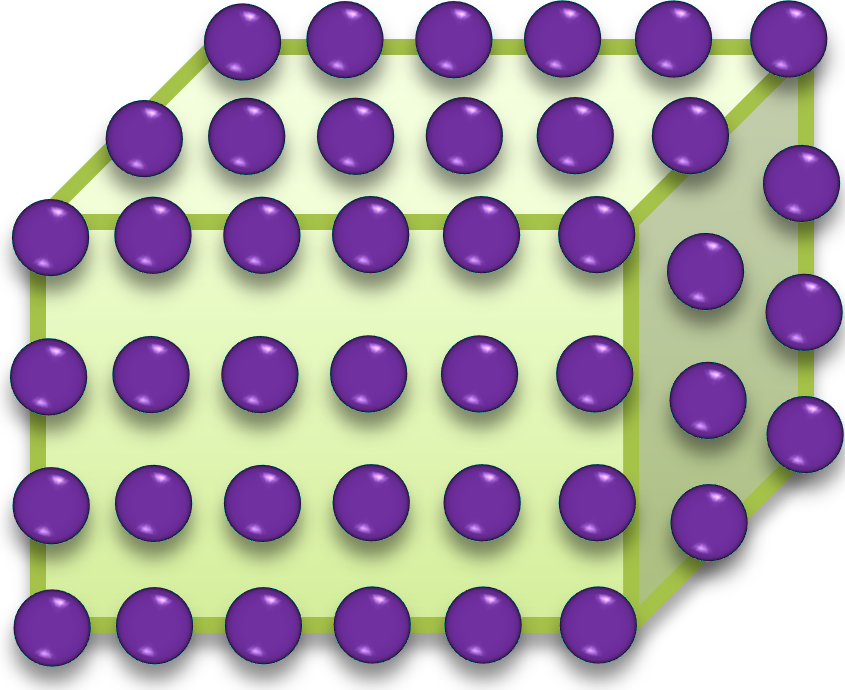
\includegraphics[width=0.5\linewidth]{Figures/NakedGridMap.png}
\caption{Grid map for fast evaluation of $e_{inter}$. Probe atoms are shown in purple.}
\label{fig:GridMap}
\end{figure}

\subsection{Optimization Algorithm}

Both idock and Vina use Monte Carlo algorithm for global optimization and Broyden-Fletcher-Goldfarb-Shanno (BFGS) \cite{786} Quasi-Newton method for local optimization. A succession of steps consisting of a mutation and a BFGS local optimization are taken, with each step being accepted according to the Metropolis criterion (Figure \ref{fig:DockingByMonteCarlo}, reprinted from \cite{493}). These steps are repeated over \textit{N} iterations, where \textit{N} correlates to the complexity of the ligand regarding number of heavy atoms and number of torsions. BFGS approximates the inverse Hessian matrix of the scoring function. It uses not only the value of the scoring function but also its gradient, which are the derivatives of the scoring function with respect to the position and orientation of the ligand, and the torsions for the active rotatable bonds in the ligand. A BFGS iteration derives a descent direction from the approximate inverse Hessian matrix, derives a step length along the descent direction by line search, and updates the approximation of inverse Hessian matrix. Both programs achieve multithreading by concurrently running multiple independent Monte Carlo tasks starting from random initial conformations.

\begin{figure}
\centering
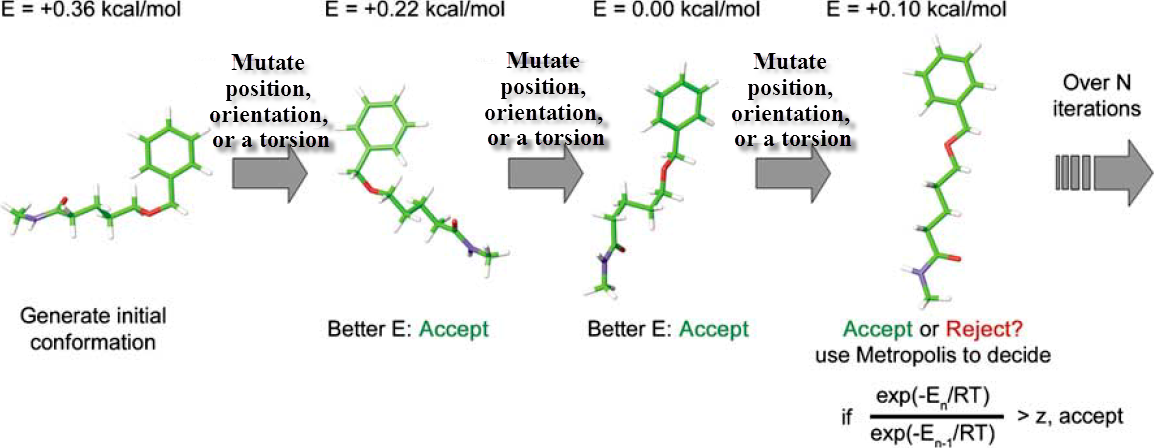
\includegraphics[width=\linewidth]{Figures/MonteCarlo.png}
\caption{Monte Carlo algorithm for docking. Figure modified from \cite{493}.}
\label{fig:DockingByMonteCarlo}
\end{figure}

Though both programs share similar optimization algorithms, their implementations differ. Compared with Vina, the Monte Carlo iterations in idock are far fewer and the BFGS iterations are more. On one hand, the fewer number of Monte Carlo iterations is compensated by a larger number of parallel Monte Carlo tasks, which is 64 by default in idock compared to 8 in Vina, guaranteeing better conformational diversity and higher CPU utilization on multi-core computers. On the other hand, the stopping criterion of BFGS local optimization does not depend on an estimated number of iterations, which is the case in Vina, but depends on the outcome of line search. The BFGS local optimization stops if and only if no appropriate step length can be obtained by line search, thus increasing the probability of finding optimal local minimums.

\subsection{Inactive Torsions}

idock automatically detects and deactivates inactive torsions, which are presented and activated in the input file in pdbqt format but have no impact on the overall scoring, such as \textemdash{OH} and \textemdash{NH$_2$}, because they only rotate the hydrogens. Figure \ref{fig:InactiveTorsions} shows an example ligand which contains 4 active torsions defined by the python script \textit{prepare\_ligand4.py} provided by AutoDock Tools \cite{785,596}. Two of them, highlighted in yellow, only rotate hydrogens and thus have no contributions to the scoring. They are re-classified as inactive torsions and deactivated while being parsed in idock. This kind of automatic detection and deactivation of inactive torsions reduces the dimension of variables to optimize in the local optimization step, leading to easier finding of local minimums.

\begin{figure}
\centering
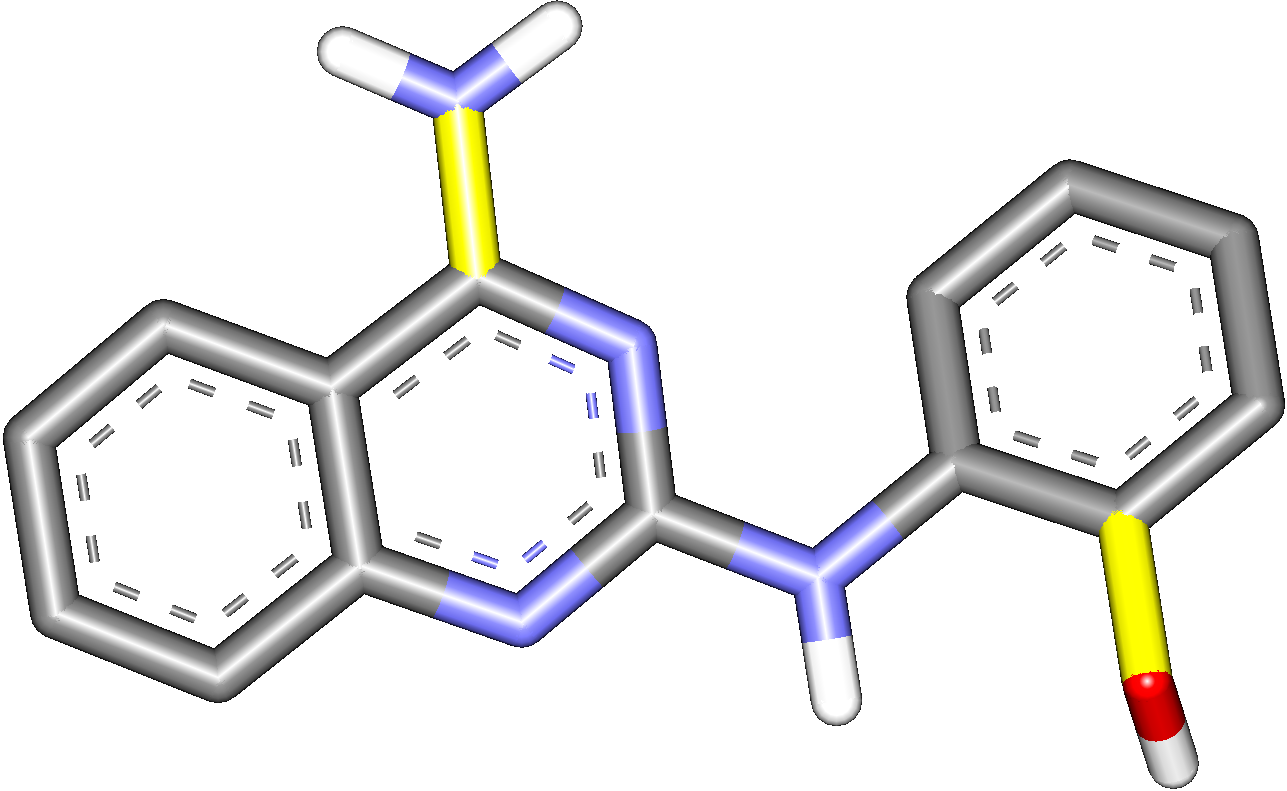
\includegraphics[width=0.5\linewidth]{Figures/ZINC00572984.png}
\caption{Example of inactive torsions highlighted in yellow. Nonpolar hydrogens are not shown for clarity.}
\label{fig:InactiveTorsions}
\end{figure}

\subsection{C++ Implementation Tricks}

idock remarkably revises the fundamental C++ implementation. idock invents its own thread pool in order to reuse threads and maintain a high CPU utilization throughout the entire screening procedure. The thread pool parallelizes the creation of grid maps and the execution of Monte Carlo tasks. idock estimates the capacity of every vector structure and intensively utilizes Rvalue reference, a new feature in the C++11 standard, to avoid frequent memory reallocation. idock flattens Vina's tree-like recursive data structure of ligand into simple linear array structure to ensure a high data cache hit rate and easy coding. idock accelerates the assignment of atom types by making use of residue information for receptor and branch information for ligand.

\section{Data}

\subsection{Proteins}

The crystal structures of HIV RT, SAHH, ADA, and PNP were collected from the Protein Data Bank (PDB) database \cite{539,537}. Protein-ligand complexes with PDB IDs of 2ZD1, 1LI4, 3IAR, and 3BGS were selected because they were crystallized at high resolutions (Table \ref{tab:SelectedPDBEntries}). Search spaces were then manually defined in cuboid shape to be large enough for ligands to freely translate and rotate inside.

\begin{table}
\centering
\begin{tabular*}
{\linewidth}
{@{\extracolsep{\fill}}ccccc}
\toprule
PDB ID & Protein & Ligand & Resolution & Box size (\AA\textsuperscript{3})\\
\midrule
2ZD1 & HIV RT & T27 & 1.80 \AA & 18 x 18 x 20\\
1LI4 & SAHH   & NAD & 2.01 \AA & 26 x 24 x 18\\
3IAR & ADA    & 3D1 & 1.52 \AA & 22 x 16 x 16\\
3BGS & PNP    & DIH & 2.10 \AA & 18 x 18 x 20\\
\bottomrule
\end{tabular*}
\caption{Selected PDB entries for HIV RT, SAHH, ADA, and PNP.}
\label{tab:SelectedPDBEntries}
\end{table}

\subsection{Ligands}

10,928 ligands were collected from the clean drug like subset of the ZINC database \cite{532}. These ligands satisfy Lipinski's \textit{Rule of Five} \cite{169} with the xLogP value of at most 5, the molecular weight between 150 Da and 500 Da, the number of hydrogen bond donors of at most 5, and the number of hydrogen bonds acceptors of at most 10.

\section{Experiments and Results}

The experiments include 1) validation of Vina and idock to ensure they are suitable for docking ligands against the four proteins, and 2) comparison of their virtual screening performance in terms of execution time, memory usage, predicted free energy, and predicted conformations.

Vina x86 version 1.1.2 and idock x86\_64 version 1.0, the most recent versions of both programs at the moment these experiments were carried out, were used for experiments. Both programs were run on desktop computers with Intel Xeon Dual Quad Core 2.4GHz and 32GB RAM under Ubuntu 10.04.1 x86\_64. The CPUs support Intel's Hyper-Threading technology, so each computer consisting of 8 physical cores can execute up to 16 logical threads simultaneously.

\subsection{Program Validation}

The four crystal ligands extracted from the four PDB complexes were conformationally randomized and redocked against their proteins by Vina and idock. Figure \ref{fig:Redocking} shows the four proteins in complex with their corresponding crystal and docked ligands. The ligands rendered in green are the crystal ones, the ligands rendered in red are the ones docked by Vina, and the ligands rendered in blue are the ones docked by idock. Table \ref{tab:RMSD} shows the root mean square deviations (RMSDs) between the crystal and docked conformations. The RMSDs are all below 2.0 \AA, a publicly accepted positive control for correct bound structure prediction, indicating both programs are suitable for docking ligands against the four proteins. The RMSDs obtained by Vina are slightly better than those obtained by idock, especially for the case of PNP. This is probably due to the coarse estimation of $e_{intra}$ in idock, which does not form covalent bonds internally but simply relies on rotatable bonds to detect atom pair mobility.

\begin{figure*}
\centering
\subfloat[HIV RT in complex with crystal and docked T27.]
{
  \label{subfig:2ZD1-T27}
  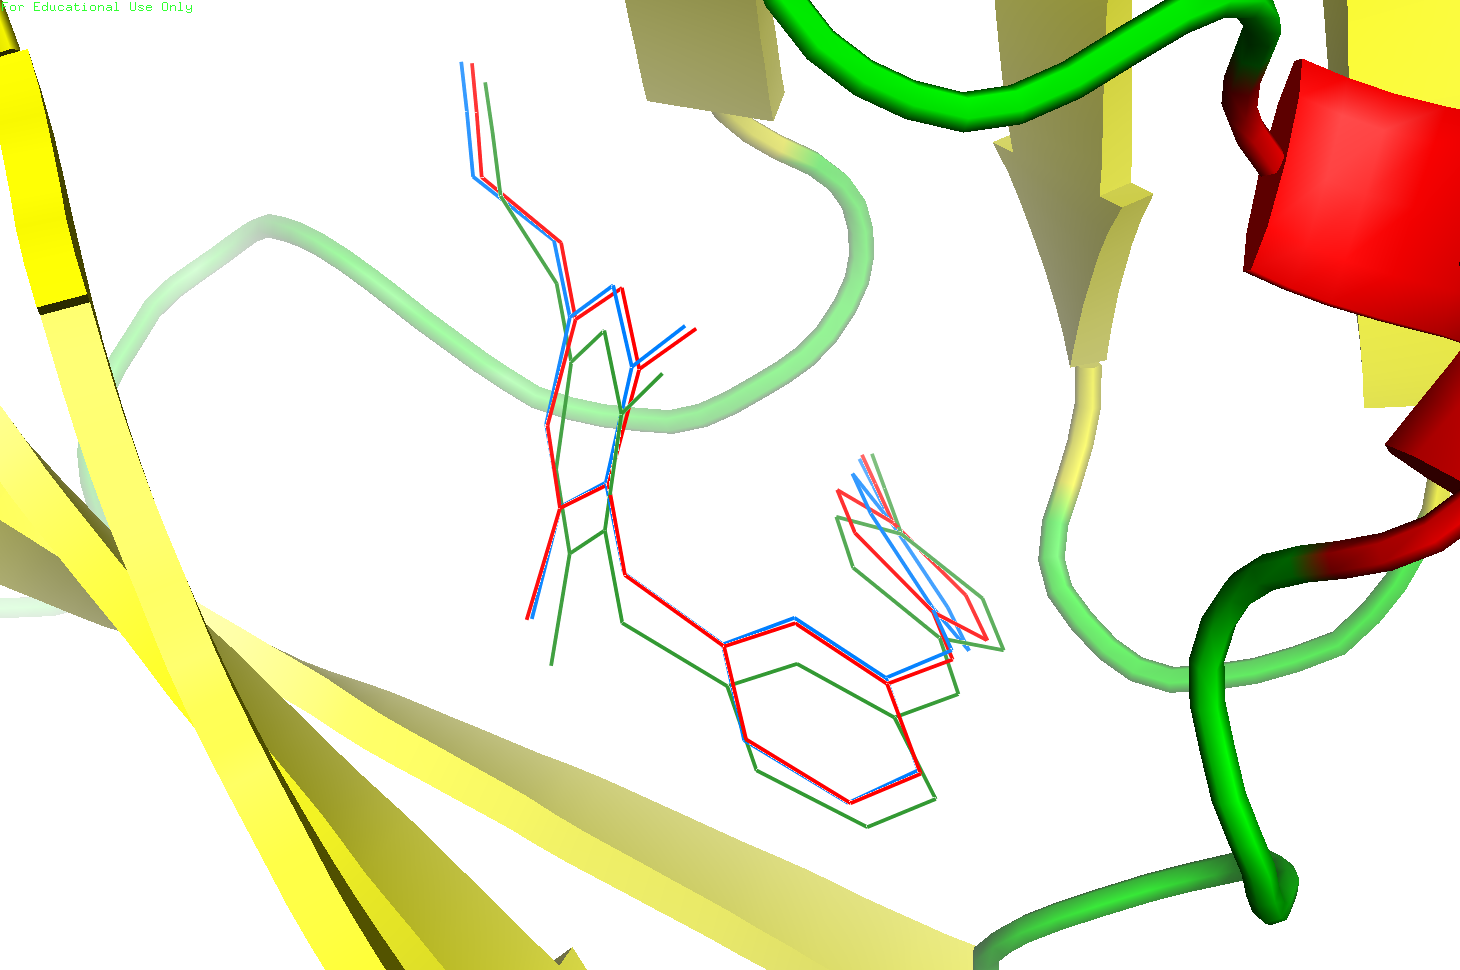
\includegraphics[width=0.236\linewidth]{Figures/2ZD1-T27.png}
}
\subfloat[SAHH in complex with crystal and docked NAD.]
{
  \label{subfig:1LI4-NAD}
  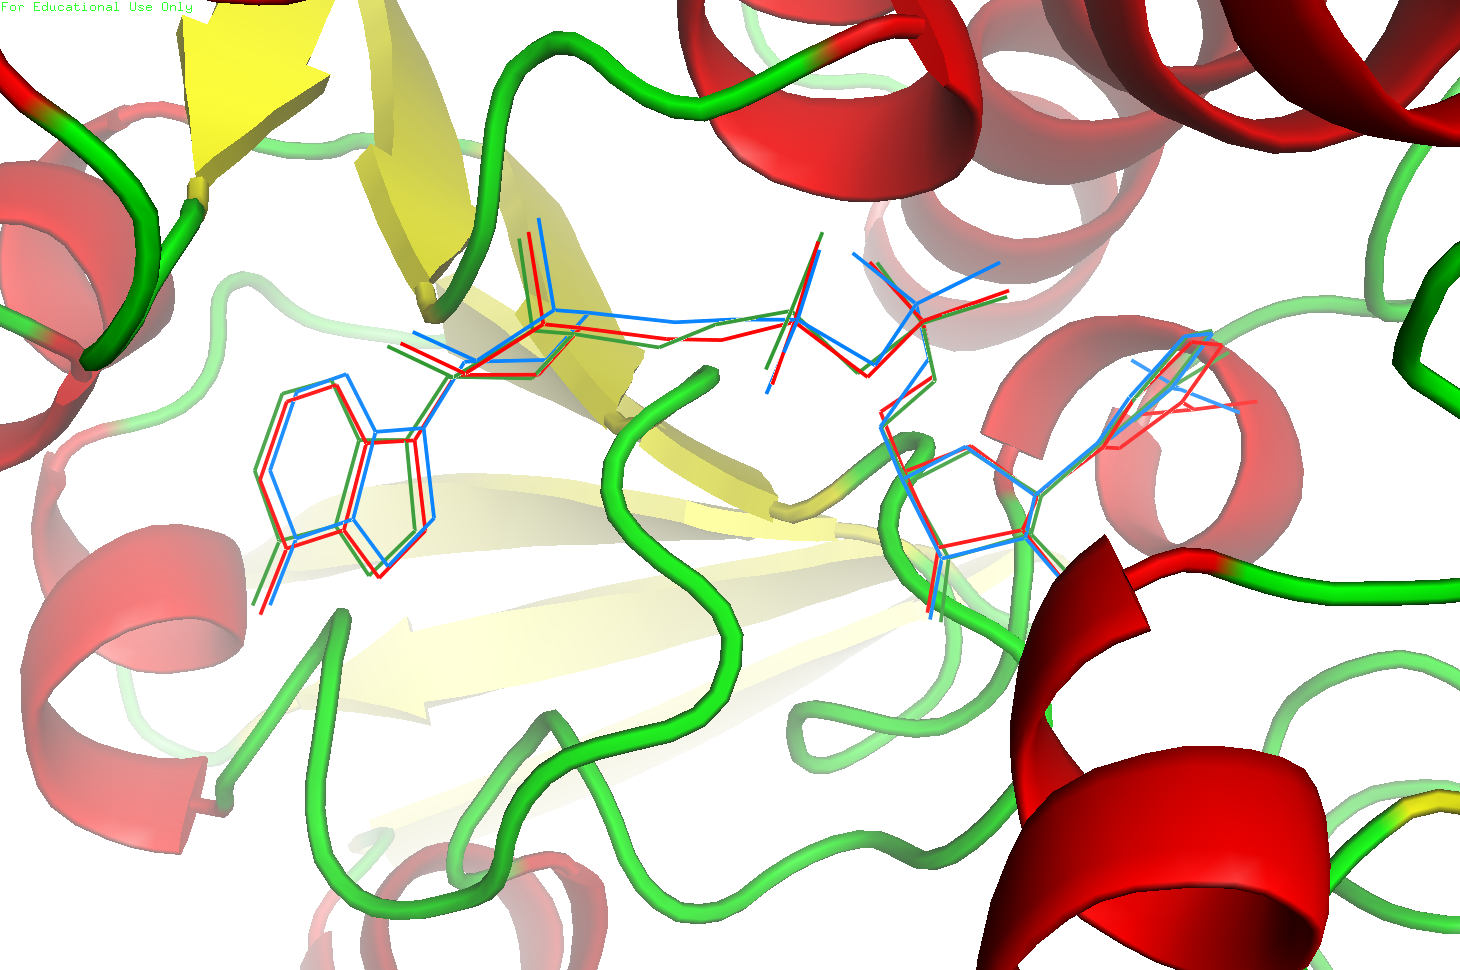
\includegraphics[width=0.236\linewidth]{Figures/1LI4-NAD.png}
}
\subfloat[ADA in complex with crystal and docked 3D1.]
{
  \label{subfig:3IAR-3D1}
  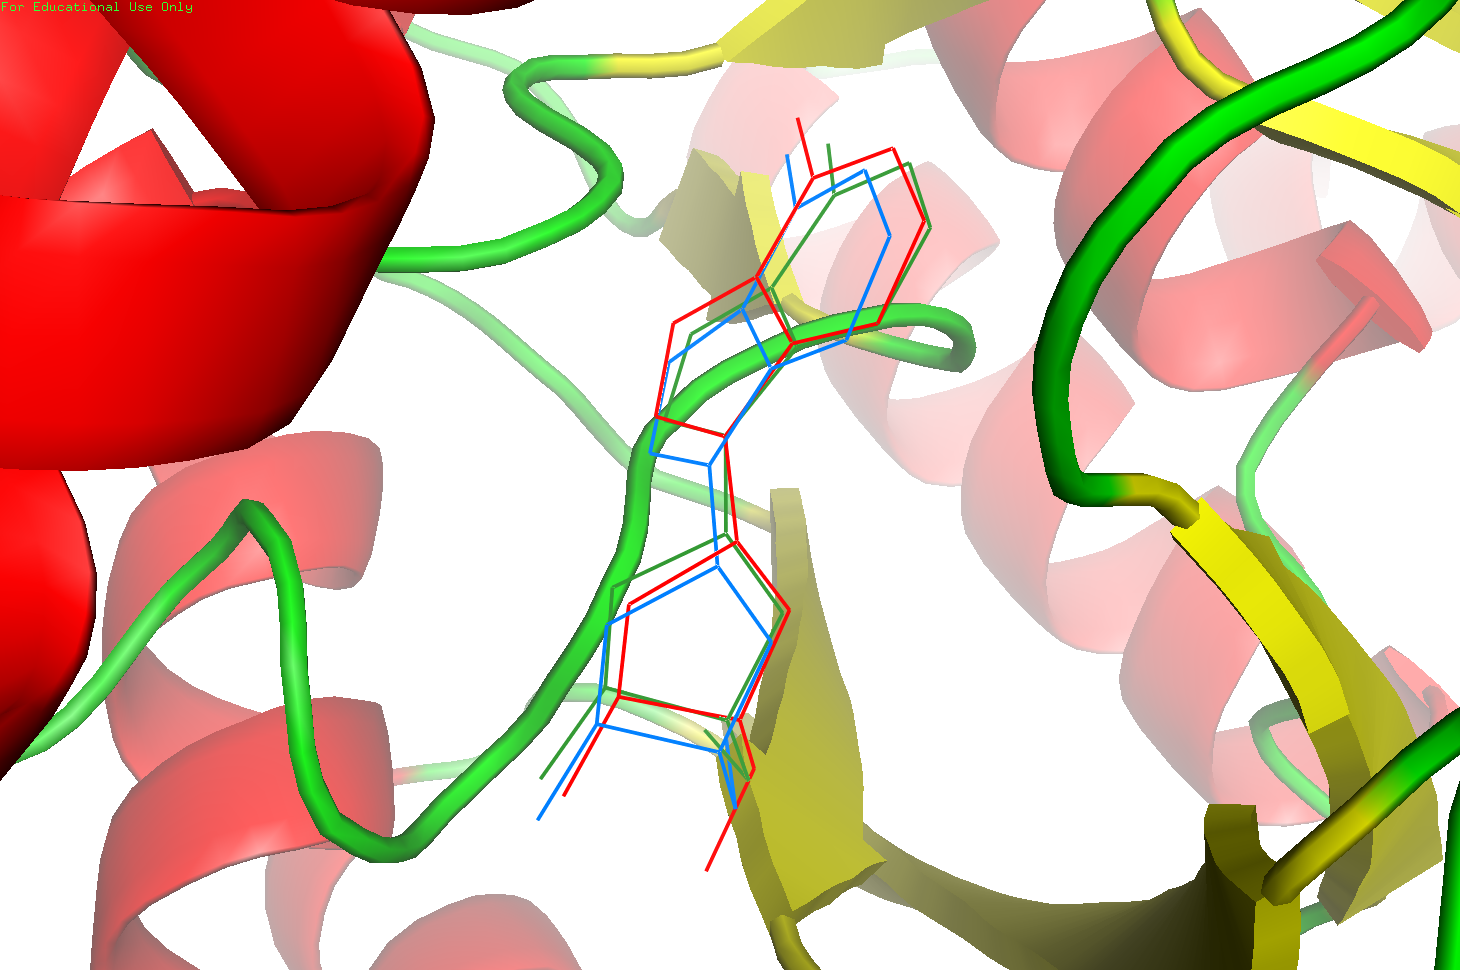
\includegraphics[width=0.236\linewidth]{Figures/3IAR-3D1.png}
}
\subfloat[PNP in complex with crystal and docked DIH.]
{
  \label{subfig:3BGS-DIH}
  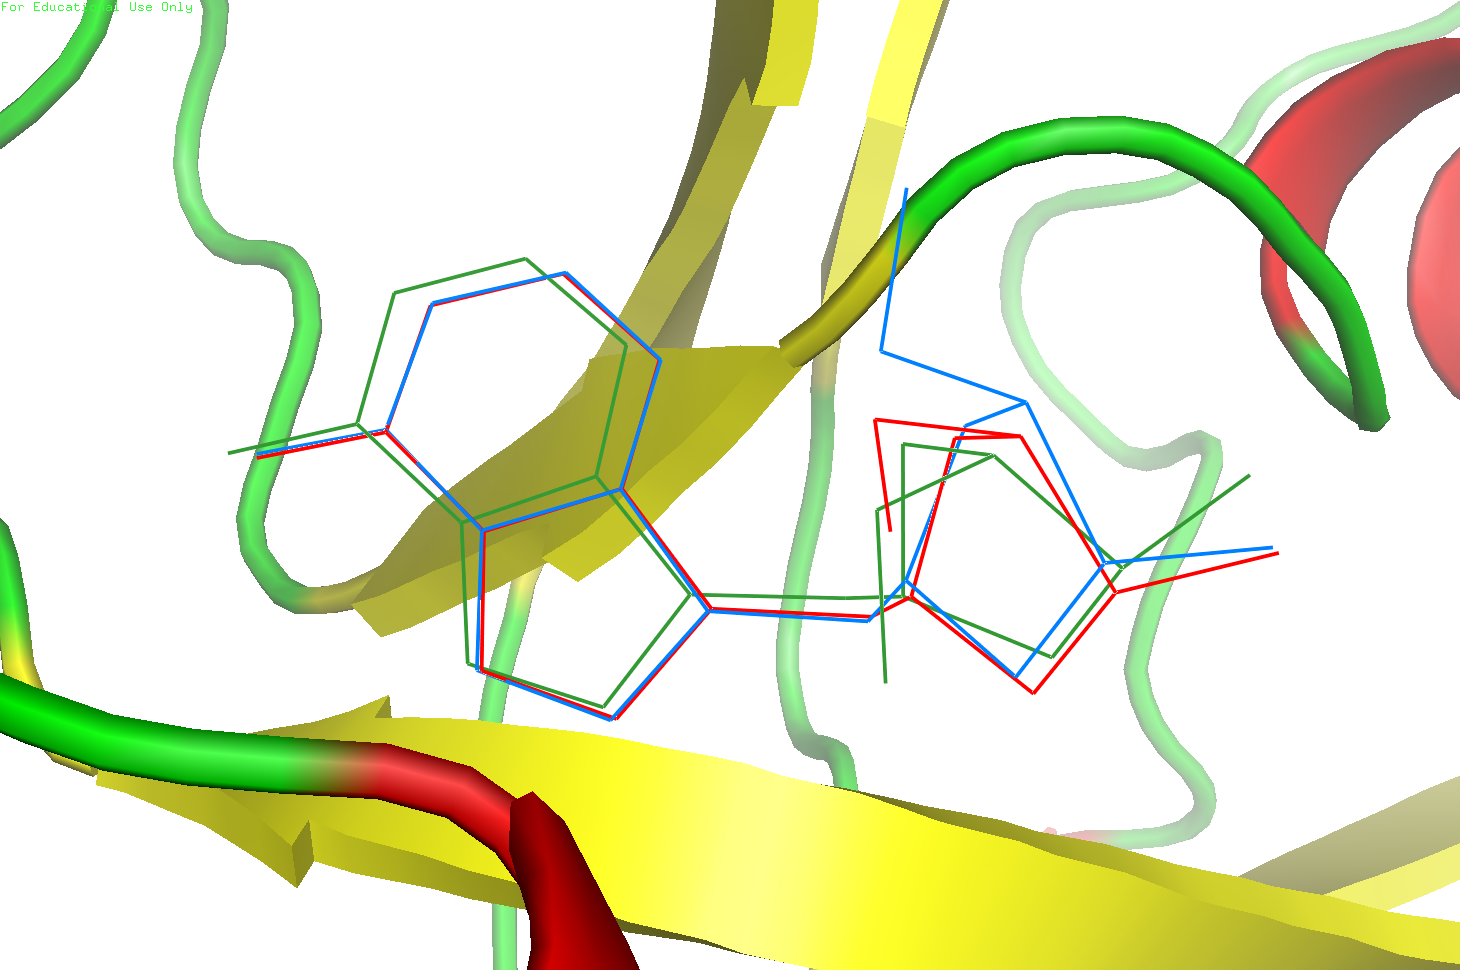
\includegraphics[width=0.236\linewidth]{Figures/3BGS-DIH.png}
}
\caption{HIV RT, SAHH, ADA, and PNP respectively in complex with crystal and docked conformations of T27, NAD, 3D1, and DIH predicted by Vina and idock.}
\label{fig:Redocking}
\end{figure*}

\begin{table}
\centering
\begin{tabular*}
{\linewidth}
{@{\extracolsep{\fill}}ccccc}
\toprule
PDB ID & Protein & Ligand & Vina (\AA) & idock (\AA)\\
\midrule
2ZD1 & HIV RT & T27 & 0.465 & 0.555\\
1LI4 & SAHH   & NAD & 0.537 & 0.593\\
3IAR & ADA    & 3D1 & 0.605 & 0.569\\
3BGS & PNP    & DIH & 0.756 & 1.170\\
\bottomrule
\end{tabular*}
\caption{RMSDs between the crystal and docked conformations of T27, NAD, 3D1, and DIH predicted by Vina and idock.}
\label{tab:RMSD}
\end{table}

\subsection{Virtual Screening}

Virtual screening was then carried out. 10,928 drug-like ligands were docked against the four proteins by Vina and idock. Since Vina can dock only one ligand in each run, a script containing 10,928 lines was generated and run instead, with each line being an execution of Vina to dock one individual ligand. Arguments to both programs were left as default. The GNU Time utility was used as profiler.

Table \ref{tab:ExecutionTimeAndMemoryUsage} compares the execution time and memory usage of both programs. Vina required 428 to 504 CPU hours for one protein case, while idock required merely 88 to 184 CPU hours, resulting in a speedup of 2.5 to 4.8 and a screening performance of 1.3 drug-like ligands per CPU minute on average. In terms of elapsed time, the speedup was increased to as high as 6.3 to 10.4 because idock better utilized the CPU cores thanks to its efficient thread pool. idock also better utilized available memory to build grid maps at a high resolution and retained them along the way. Even though idock consumed more memory than Vina, its maximum resident set size did not exceed 1.5 GB, hence idock can run be on mainstream desktop computers.

\begin{table}
\centering
\begin{tabular*}
{\linewidth}
{@{\extracolsep{\fill}}rrrrr}
\toprule
Program & CPU Hours & Elapsed & CPU Util. & Max Mem Usage\\
\midrule
\multicolumn{5}{l}{\textbf{HIV RT}}\\
Vina  & 464 & 69:15:13 &  670\% & 126 MB\\
idock & 162 & 10:57:46 & 1474\% & 856 MB\\
Ratio & 2.9 &      6.3 & 0.45   & 0.15\\
\noalign{\smallskip\smallskip}
\multicolumn{5}{l}{\textbf{SAHH}}\\
Vina  & 460 & 78:53:59 &  582\% &   150 MB\\
idock & 184 & 12:24:24 & 1484\% & 1,368 MB\\
Ratio & 2.5 &      6.4 &  0.39  & 0.11\\
\noalign{\smallskip\smallskip}
\multicolumn{5}{l}{\textbf{ADA}}\\
Vina  & 504 & 74:22:37 &  677\% & 114 MB\\
idock & 127 &  8:46:12 & 1452\% & 764 MB\\
Ratio & 4.0 &      8.5 &  0.47  & 0.15\\
\noalign{\smallskip\smallskip}
\multicolumn{5}{l}{\textbf{PNP}}\\
Vina  & 428 & 62:19:55 &  687\% & 116 MB\\
idock &  88 &  5:58:19 & 1479\% & 857 MB\\
Ratio & 4.8 &     10.4 &  0.46  & 0.13\\
\noalign{\smallskip\smallskip}
\multicolumn{5}{l}{\textbf{Average}}\\
Vina  & 464 & 71:12:56 &  654\% & 124 MB\\
idock & 140 &  9:31:40 & 1472\% & 961 MB\\
Ratio & 3.3 &      7.5 & 0.44   & 0.13\\
\bottomrule
\end{tabular*}
\caption{Execution time and memory usage of docking 10,928 drug-like ligands against HIV RT, SAHH, ADA, and PNP by Vina and idock. Maximum CPU utilization is 1600\% due to Intel's Hyper-Threading technology.}
\label{tab:ExecutionTimeAndMemoryUsage}
\end{table}

Table \ref{tab:RMSEAndRMSD} summarizes the root mean square errors (RMSEs) of free energies and RMSDs of conformations predicted by both programs. The RMSEs of free energies predicted by both programs vary from 0.31 to 0.46 kcal/mol, apparently less than 2.85 kcal/mol, the standard error obtained by Vina, indicating both programs predicted very similar free energies. For 27\% to 40\% of all the 10,928 ligands, the RMSD of the conformations predicted by both programs is equal to or less than 1.0 \AA, and for 49\% to 61\%, the RMSD is equal to or less than 2.0 \AA, indicating both programs predicted similar conformations for around half of the cases.

\begin{table}
\centering
\begin{tabular*}
{\linewidth}
{@{\extracolsep{\fill}}cccc}
\toprule
Protein & RMSE (kcal/mol) & Avg RMSD (\AA) & RMSD $\leq$ 2.0 \AA\\
\midrule
HIV RT & 0.35 & 2.554 & 61\%\\
SAHH   & 0.46 & 4.190 & 49\%\\
ADA    & 0.33 & 2.620 & 59\%\\
PNP    & 0.31 & 2.966 & 53\%\\
\bottomrule
\end{tabular*}
\caption{RMSEs of free energies and RMSDs of conformations predicted by Vina and idock.}
\label{tab:RMSEAndRMSD}
\end{table}

In order to shortlist a few promising ligands that bind to HIV RT with a high affinity but bind to SAHH, ADA, and PNP with a low affinity, filtering criteria were set. Ligands whose predicted free energies against HIV RT are below or equal to -11.0 kcal/mol and whose predicted free energies against the other three proteins are above or equal to -8.5 kcal/mol were shortlisted in Table \ref{tab:ShortlistedLigands}. The ZINC19888543 predicted by Vina and the ZINC44392991 predicted by idock were further investigated. Table \ref{tab:ZINC19888543-ZINC44392991} cites their predicted xLogP, number of hydrogen bond donors (HBD), number of hydrogen bond acceptors (HBA), molecular weight (MW), and number of rotatable bonds (NRB) from the ZINC database \cite{532}. Figures \ref{fig:Vina-ZINC19888543} and \ref{fig:idock-ZINC44392991}, rendered by PoseView 1.0.0 \cite{748}, show their predicted binding conformations in complex with the four proteins. Hydrogen bonds, salt bridges and metal interactions are highlighted as black dashed lines. Hydrophobic interactions are highlighted as green solid lines. Pi-Pi and Pi-cation interactions are highlighted as green dashed lines. It can be seen that ZINC19888543 interacts with HIV RT mainly through hydrophobic effects and Pi-Pi interactions, while ZINC44392991 interacts with HIV RT mainly through Pi-Pi interactions and hydrogen bonding.

\begin{table}
\centering
\begin{tabular*}
{\linewidth}
{@{\extracolsep{\fill}}ccccc}
\toprule
Ligand & HIV RT & SAHH & ADA & PNP\\
\midrule
\multicolumn{5}{l}{\textbf{Vina}}\\
ZINC04667184 & -11.1 & -6.6 & -7.5 & -7.5\\
ZINC06720921 & -11.0 & -7.4 & -8.0 & -8.4\\
ZINC14545253 & -11.0 & -6.5 & -8.0 & -7.6\\
ZINC19888543 & -11.1 & -7.9 & -7.8 & -7.8\\
ZINC26423182 & -11.1 & -6.4 & -7.8 & -7.4\\
ZINC49453017 & -11.3 & -7.1 & -8.3 & -7.6\\
ZINC60603133 & -11.0 & -7.9 & -8.3 & -7.4\\
\noalign{\smallskip\smallskip}
\multicolumn{5}{l}{\textbf{idock}}\\
ZINC03012460 & -11.3 & -8.3 & -7.8 & -7.3\\
ZINC04667184 & -11.2 & -7.6 & -7.7 & -8.0\\
ZINC44392991 & -11.1 & -7.7 & -7.3 & -8.1\\
ZINC49453017 & -11.6 & -7.3 & -8.3 & -7.8\\
\bottomrule
\end{tabular*}
\caption{Shortlisted ligands whose predicted free energies against HIV RT are below or equal to -11.0 kcal/mol and whose predicted free energies against the other three proteins are above or equal to -8.5 kcal/mol.}
\label{tab:ShortlistedLigands}
\end{table}

\begin{table}
\centering
\begin{tabular*}
{\linewidth}
{@{\extracolsep{\fill}}cccccc}
\toprule
Ligand & xLogP & HBD & HBA & MW (Da) & NRB\\
\midrule
ZINC19888543 & 4.48 & 1 & 3 & 342 & 3\\
ZINC44392991 & 4.24 & 1 & 6 & 391 & 6\\
\bottomrule
\end{tabular*}
\caption{Chemical properties of ZINC19888543 predicted by Vina and ZINC44392991 predicted by idock.}
\label{tab:ZINC19888543-ZINC44392991}
\end{table}

\begin{figure*}
\centering
\subfloat[HIV RT in complex with ZINC19888543.]
{
  \label{subfig:2ZD1-ZINC19888543}
  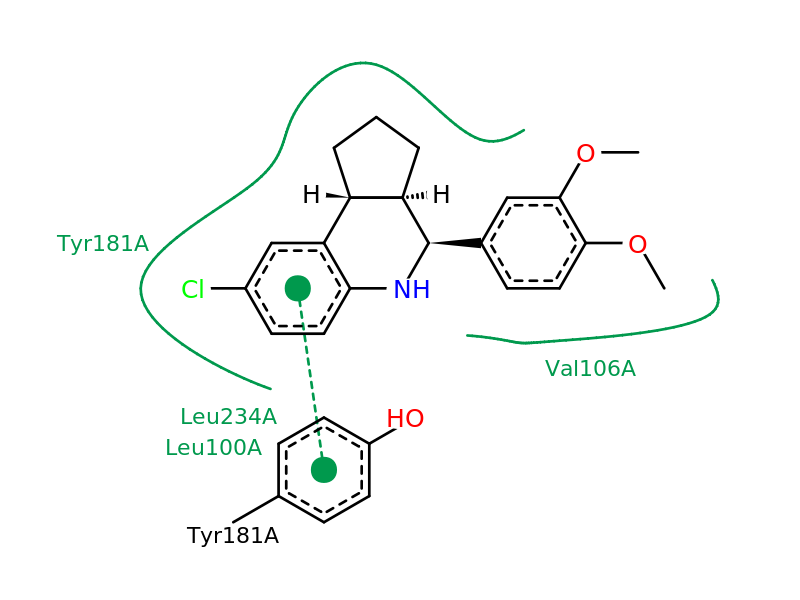
\includegraphics[width=0.236\linewidth]{Figures/2ZD1-ZINC19888543.png}
}
\subfloat[SAHH in complex with ZINC19888543.]
{
  \label{subfig:1LI4-ZINC19888543}
  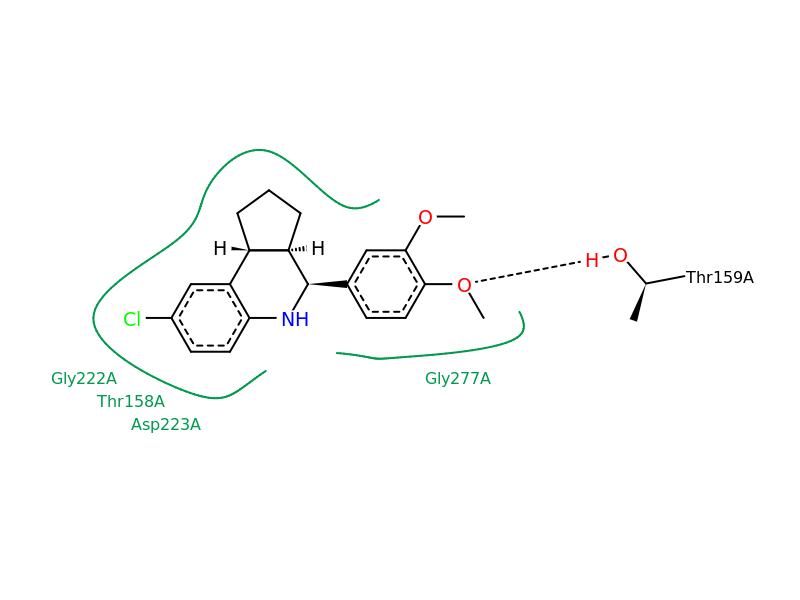
\includegraphics[width=0.236\linewidth]{Figures/1LI4-ZINC19888543.png}
}
\subfloat[ADA in complex with ZINC19888543.]
{
  \label{subfig:3IAR-ZINC19888543}
  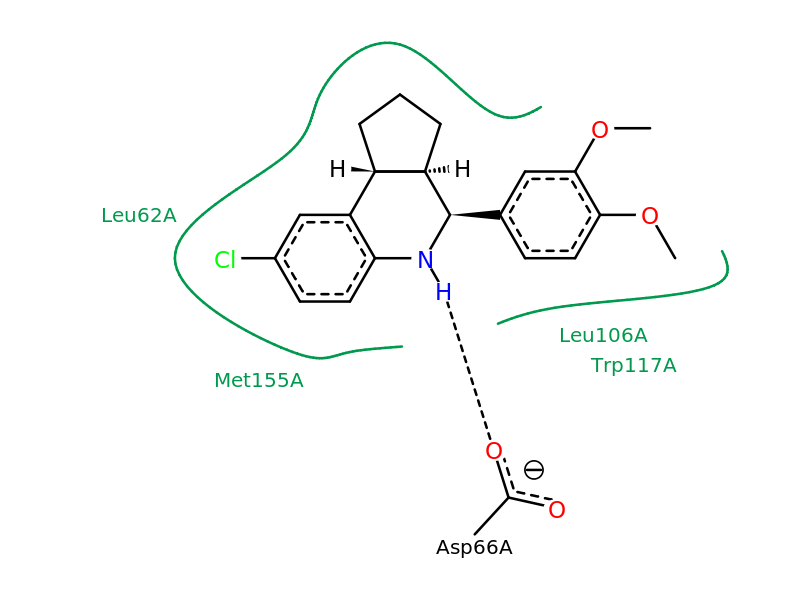
\includegraphics[width=0.236\linewidth]{Figures/3IAR-ZINC19888543.png}
}
\subfloat[PNP in complex with ZINC19888543.]
{
  \label{subfig:3BGS-ZINC19888543}
  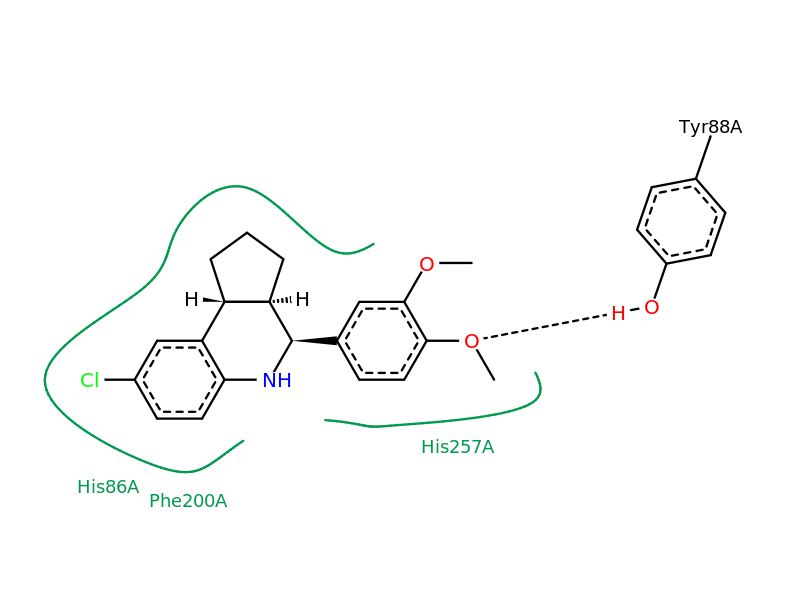
\includegraphics[width=0.236\linewidth]{Figures/3BGS-ZINC19888543.png}
}
\caption{HIV RT, SAHH, ADA, and PNP in complex with ZINC19888543 docked by Vina.}
\label{fig:Vina-ZINC19888543}
\end{figure*}

\begin{figure*}
\centering
\subfloat[HIV RT in complex with ZINC44392991.]
{
  \label{subfig:2ZD1-ZINC44392991}
  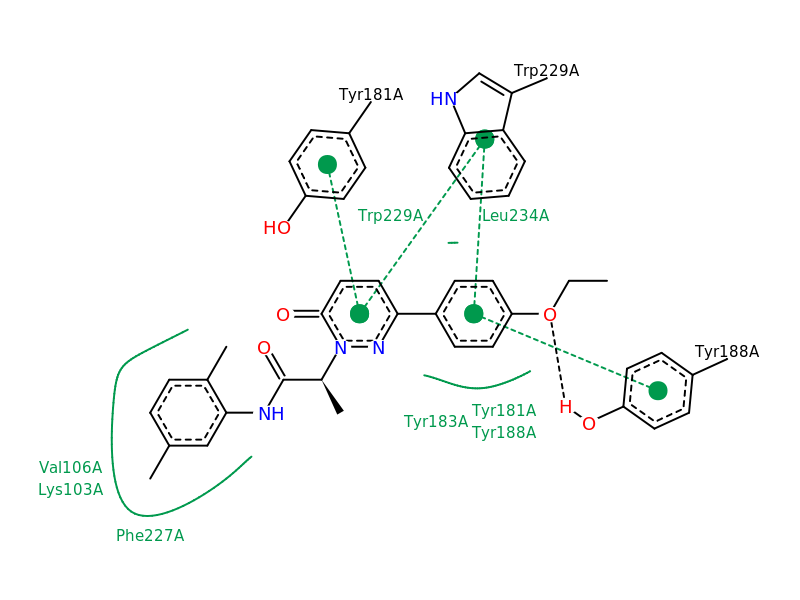
\includegraphics[width=0.236\linewidth]{Figures/2ZD1-ZINC44392991.png}
}
\subfloat[SAHH in complex with ZINC44392991.]
{
  \label{subfig:1LI4-ZINC44392991}
  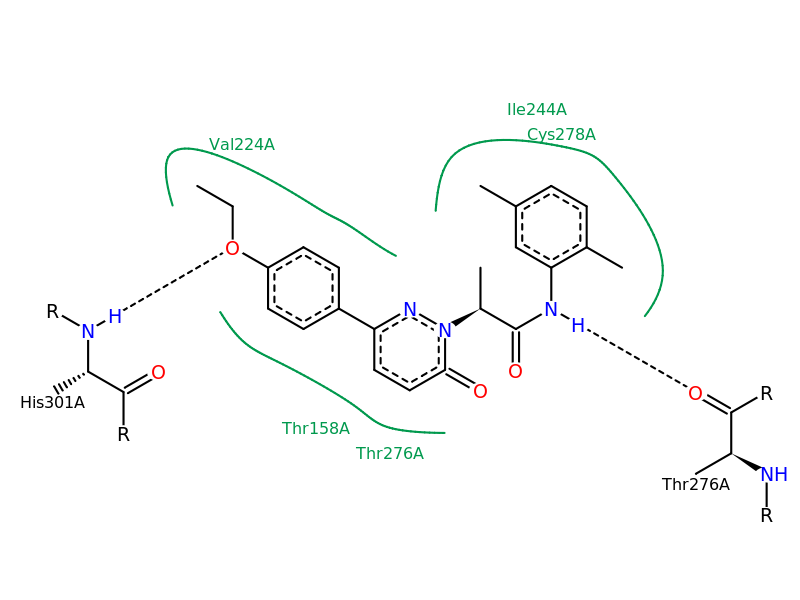
\includegraphics[width=0.236\linewidth]{Figures/1LI4-ZINC44392991.png}
}
\subfloat[ADA in complex with ZINC44392991.]
{
  \label{subfig:3IAR-ZINC44392991}
  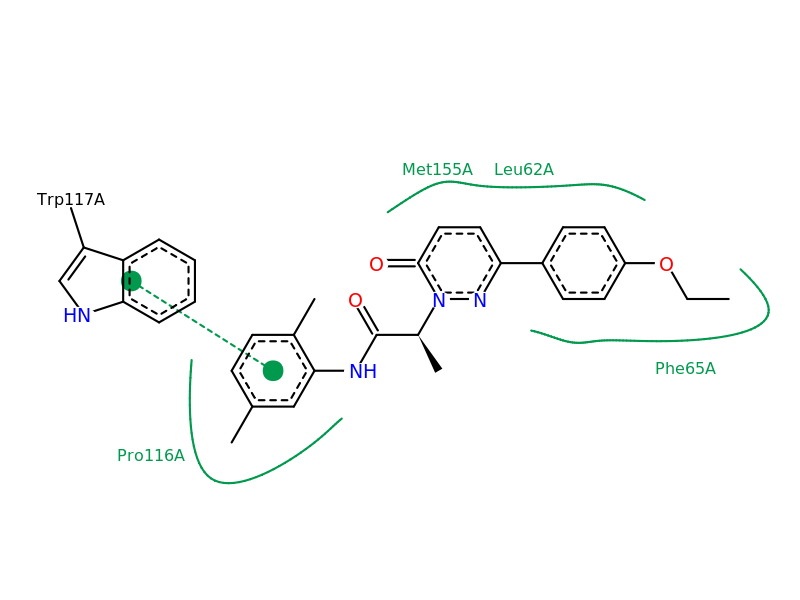
\includegraphics[width=0.236\linewidth]{Figures/3IAR-ZINC44392991.png}
}
\subfloat[PNP in complex with ZINC44392991.]
{
  \label{subfig:3BGS-ZINC44392991}
  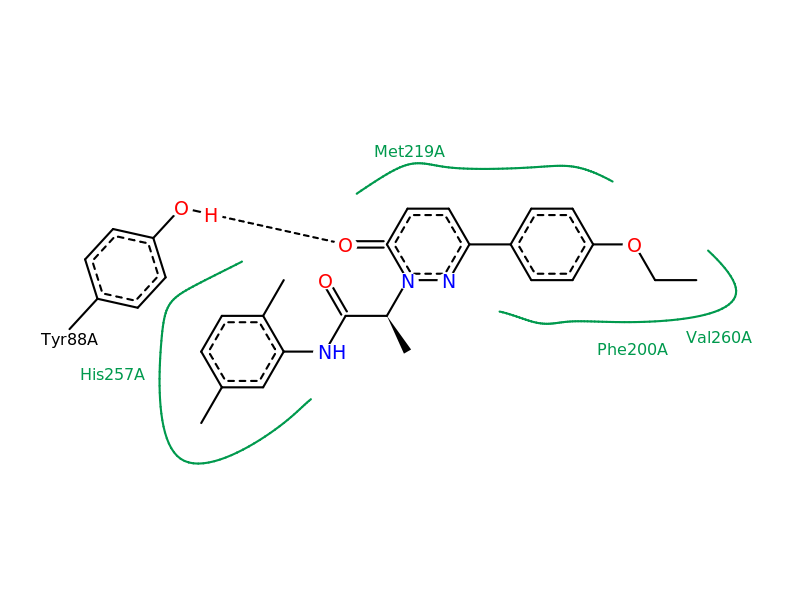
\includegraphics[width=0.236\linewidth]{Figures/3BGS-ZINC44392991.png}
}
\caption{HIV RT, SAHH, ADA, and PNP in complex with ZINC44392991 docked by idock.}
\label{fig:idock-ZINC44392991}
\end{figure*}

\section{Discussion}

Both Vina and idock adopt the same scoring function. They differ in their C++ implementations, data structures, numerical models, and Monte Carlo algorithms. idock implements its own thread pool to maintain a high CPU utilization throughout the entire screening procedure. It intensively utilizes modern C++11 techniques, particularly Rvalue references to avoid frequent reallocations of array data. It flattens Vina's tree-like recursive data structures into simple array structures to guarantee a high data cache hit rate. It automatically detects and deactivates inactive torsions and thus reduces the dimension of variables to optimize.

In Vina's official forum, there are tremendous requests for the support for virtual screening. The development of idock perfectly complements Vina. idock has built-in support for virtual screening. It searches for ligands in a user-specified folder and docks them one by one. It reuses threads and grid maps across multiple ligands. idock has very similar input and output arguments as Vina, so it should be quite easy for existing Vina users to transit to idock. Vina supports flexible receptor docking by rotating flexible side-chains. However, we have not yet implemented flexible receptor docking into idock at the moment, so users who need this kind of docking should refer to Vina.

\section{Availability}

idock is open source under Apache License 2.0 and is freely available at https://GitHub.com/HongjianLi/idock. Precompiled executables for 32-bit and 64-bit Linux, Windows, Mac OS X and FreeBSD are provided. Docking examples and API documentations are also provided.

\section{Conclusion}

We have developed idock, a multithreaded structure-based virtual screening tool for flexible ligand docking. It is capable of screening 1.3 drug-like ligands per CPU minute on average, making it a very competitive tool. Compared with Vina, idock achieves a speedup of 3.3 in terms of CPU time and a speedup of 7.5 in terms of elapsed time on average. But even so, it still required about 10 hours on average to dock 10,928 drug-like ligands against a certain protein, not to mention massive docking of millions of ligands. Virtual screening remains a time-consuming practice. Faster algorithms and implementations are highly desired. Porting idock to GPU using CUDA is one of our future directions.

\bibliographystyle{unsrtnat}
\bibliography{../refworks}

\end{document}
